%%%%%%%%%%%%%%%%%%%%%
% Short Sectioned Assignment
% LaTeX Template
% Version 1.0 (5/5/12)
%
% This template has been downloaded from:
% http://www.LaTeXTemplates.com
%
% Original author:
% Frits Wenneker (http://www.howtotex.com)
%
% License:
% CC BY-NC-SA 3.0 (http://creativecommons.org/licenses/by-nc-sa/3.0/)
%
%%%%%%%%%%%%%%%%%%%%%

%----------------------------------------------------------------------------------------
%	PACKAGES AND OTHER DOCUMENT CONFIGURATIONS
%----------------------------------------------------------------------------------------

\documentclass[paper=a4, fontsize=11pt]{scrartcl} % A4 paper and 11pt font size

\usepackage{graphicx}
\usepackage[T1]{fontenc} % Use 8-bit encoding that has 256 glyphs
\usepackage{fourier} % Use the Adobe Utopia font for the document - comment this line to return to the LaTeX default
\usepackage[english]{babel} % English language/hyphenation
\usepackage{amsmath,amsfonts,amsthm} % Math packages

\usepackage{lipsum} % Used for inserting dummy 'Lorem ipsum' text into the template

\usepackage{sectsty} % Allows customizing section commands
\allsectionsfont{\centering \normalfont\scshape} % Make all sections centered, the default font and small caps

\usepackage{fancyhdr} % Custom headers and footers
\pagestyle{fancyplain} % Makes all pages in the document conform to the custom headers and footers
\fancyhead{} % No page header - if you want one, create it in the same way as the footers below
\fancyfoot[L]{} % Empty left footer
\fancyfoot[C]{} % Empty center footer
\fancyfoot[R]{\thepage} % Page numbering for right footer
\renewcommand{\headrulewidth}{0pt} % Remove header underlines
\renewcommand{\footrulewidth}{0pt} % Remove footer underlines
\setlength{\headheight}{13.6pt} % Customize the height of the header

\numberwithin{equation}{section} % Number equations within sections (i.e. 1.1, 1.2, 2.1, 2.2 instead of 1, 2, 3, 4)
\numberwithin{figure}{section} % Number figures within sections (i.e. 1.1, 1.2, 2.1, 2.2 instead of 1, 2, 3, 4)
\numberwithin{table}{section} % Number tables within sections (i.e. 1.1, 1.2, 2.1, 2.2 instead of 1, 2, 3, 4)

\setlength\parindent{0pt} % Removes all indentation from paragraphs - comment this line for an assignment with lots of text

%----------------------------------------------------------------------------------------
%	TITLE SECTION
%----------------------------------------------------------------------------------------

\newcommand{\horrule}[1]{\rule{\linewidth}{#1}} % Create horizontal rule command with 1 argument of height

\title{	
\normalfont \normalsize 
\textsc{CS 472 Evolutionary Computation} \\ [25pt] % Your university, school and/or department name(s)
\horrule{0.5pt} \\[0.4cm] % Thin top horizontal rule
\huge Project 2 \\ % The assignment title
\horrule{2pt} \\[0.5cm] % Thick bottom horizontal rule
}

\author{Alex Cochrane} % Your name

\date{\normalsize\today} % Today's date or a custom date

\begin{document}

\maketitle % Print the title

%------------------------------------------------

%\horrule{0.5pt} \\[0.4cm] % Thin top horizontal rule
\section{Abstract}

%------------------------------------------------

\paragraph{} For this project we were tasked with adding functionality to create a Genetic Program that had certain functionality and could easily be expanded upon later. Doing this in C++ I chose to do the typing of individual nodes through polymorphism and inheritance. I decided it would be easiest to build my individuals up as abstract nodes. The nodes themselves will be typed off of there operation. Therefore when I build my populations of individuals I really just have to build a population of nodes and I will not have to worry about their types.

%------------------------------------------------

\horrule{0.5pt} \\[0.4cm] % Thin top horizontal rule
\section{Algorithm and Individual Description}

%------------------------------------------------
\paragraph{} For now there are only operations for building up a population of individuals, getting there fitness and removing/copying them. The easiest way to show how these methods work is to show the class diagram for there creation and then do pseudo code for the functions that need an explanation. This class diagram shows both how individuals, or nodes in my code, are formed and structured as well as the population of individuals. Helper functions under population to call functions for individuals are not shown in the diagram because at the time of its creation, the semantics of how I was going to handle them were not done yet.

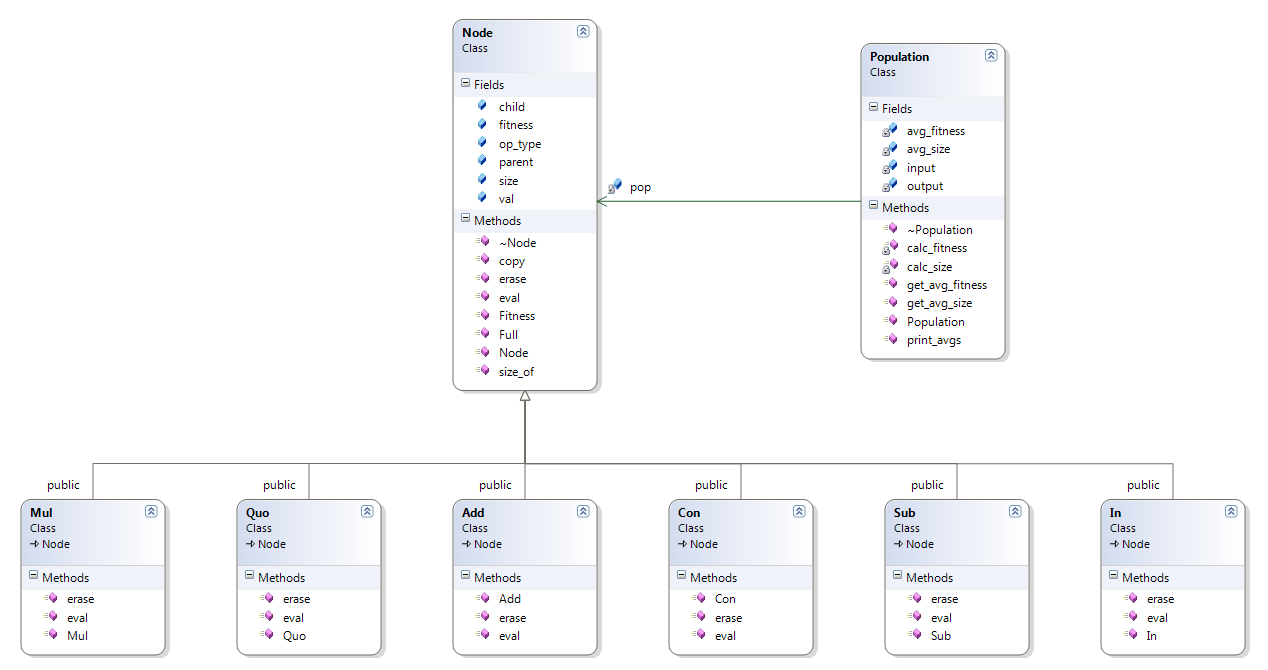
\includegraphics[scale=.5]{ClassDiagram}

\paragraph{} As the diagram shows, each node has the capability of being an addition, subtraction, multiplication, division, constant, and an input. The general attributes of a Node are its fitness, size, children, parent, and for certain individuals average fitness, average size, and value are necessary. These attributes are set by functions and will be discussed more during the following algorithm descriptions.

\paragraph{Pseudo Code: Copy}
\begin{verbatim}
while ( Individual[]->fitness > 0.01 ) //larger then the smallest value measured
    if( repeated fitness 100 times || 1000 generations have been created)
        break
    while( next Population is not filled )
        create a new individual to put in the population
        randomly select an individual from the current population N = 5 times
        select the one with the best fitness and make the new individual it
    crossover
    mutate
    calculate the new fitness / sort
\end{verbatim}

\paragraph{} DO NOT KNOW YET

\paragraph{Pseudo Code: Evaluate}
\begin{verbatim}
// if non term
return eval(child[0]) op eval(child[1]); // where op is the operator based off of which node we are in
// if const
return val; // Our constant value
// if input
return in; // return the input value for evaluation
\end{verbatim}

\paragraph{} For evaluation of non terminals we want to return the evaluation of the right and left branches of the tree using the op for what node it is to perform an operation on the two returned values. If it is a constant we return a constant value generated on creation of the tree and if we are input we return the value of the input given on the call to evaluation.

\paragraph{Pseudo Code: Erase}
\begin{verbatim}
// if non term
while all children are deleted
    child->erase();
    increment;
delete this;
return;
// if const or input
delete this; // we don't have children
return;
\end{verbatim}

\paragraph{} If we are a non terminal we need to erase our children. If we are a constant or an input we can just delete ourselves and return because we have no children.

\paragraph{Pseudo Code: Size}
\begin{verbatim}
temp = 1; // size
while all children have not been looked at
    if( child != NULL )
        temp += size( child );
    else // child == NULL const or input
        temp = 1;
size = temp; // local assignment so it is saved in the node/individual
return temp; // this returns so we can calculate
\end{verbatim}

\paragraph{} The essence of this code is that it uses recursion to go down to the end nodes and build up the size from the bottom. To calculate an average size then we just need to touch each node and average out those size values which are then stored at the head node. If the node is a constant or input node, we can say it is of size one and start returning up our recursive calls that were made when we were non terminals.

\paragraph{Pseudo Code: Full}
\begin{verbatim}
parent = node // this is the node passed in

if depth is not greater then our max depth
    while all children are filled
        generate a random individual // Add,Sub,...
\end{verbatim}

\paragraph{} 

%------------------------------------------------

\horrule{0.5pt} \\[0.4cm] % Thin top horizontal rule
\section{Results}

%------------------------------------------------



%------------------------------------------------

\horrule{0.5pt} \\[0.4cm] % Thin top horizontal rule
\section{Conclusion}

%------------------------------------------------
\paragraph{} The Genetic Algorithm seems to be working well in the since that it is taking good individuals and mutating them along with crossover to get a better next generation. The problem with this solution however is that a great individual is not present in the population at the start. Without this individual that is almost at the minimum at the start, it is very unlikely to actually find the global minimum.

\paragraph{} Some improvements that could have been done were to add an individual to the population that was not random but was in fact very close to the actual minimums vector/fitness. This would guarantee that I had an individual that would be able to move to the minimum. This does take away from the whole purpose of the GA but as stated before, it guarantees a solution is found.

\paragraph{} While it would be interesting to get these problems to all work correctly, the run time for them with 1000 individuals in the population takes quite some time. Each fix could take up to 5 minutes to run that fix to see if an improvement was made. Therefore I would like to rewrite the way I do sorting a bit but as just an exercise I have learned quite a bit about GA's and how they operate. The most interesting bit was the affect or the mutation ratio as well as the likely hood for crossover to occur. Changing these values had the greatest affect on the shape as the graph as well. The lower the mutation value was the more linear the graph looked which is why most of these graphs are linear. The values took a steep initial two or three steps and then hill climbed as a group to a minima.

\paragraph{} Crossover had this same affect. The more likely two individuals were to crossover, the slower it took to hill climb. This is because good individuals are not always taken. Especially without elitism in the GA, it was difficult to assume that the best individual always stayed. Nonetheless it worked out to were the algorithms were working well together to at least find minima and with more tweaking of values and intervals it is plausible to think that the global minimum would eventually be found.
%------------------------------------------------

\horrule{0.5pt} \\[0.4cm] % Thin top horizontal rule
\end{document}
